\documentclass[a4paper, 12pt]{article}

% <--------- Packages ---------> %

\usepackage{fullpage}   % Package to use full page
\usepackage{tikz}       % Package for drawing
\usepackage{pdfpages}
\usepackage{fancyhdr}
\usepackage{array}
\usepackage{tabularx}
\usepackage{colortbl}
\usepackage{pgfplots}
\usepackage{xcolor}
\usepackage{float}

% <--------- Mathematics ---------> %

\usepackage{amssymb}   % Extra symbols
\usepackage{amsthm}  
\usepackage{amsmath}   % Theorem-like environments
\usepackage{thmtools}  % Theorem-like environments
\usepackage{mathtools} % Fonts and environments for mathematical formuale
\usepackage{mathrsfs}  % Script font with \mathscr{}

% <--------- Others ---------> %

\usepackage{indentfirst}
\usepackage[utf8]{inputenc}
\usepackage[english]{babel}
\usepackage[thinlines]{easytable}
\usepackage{caption}
% \usepackage[parfill]{parskip}
\usepackage{pgfplots}


%===========================================%
%=            Page Style                   =%

\usepackage{times}

\pgfplotsset{compat=1.7}
\setlength{\parindent}{1.3em}
\renewcommand{\baselinestretch}{1.5}

%=                                         =%
%===========================================%


%===========================================%
%=            Code Setup                   =%

\usepackage{listings}
\usepackage{color}

\definecolor{dkgreen}{RGB}{163, 190, 140}
\definecolor{gray}{RGB}{59, 66, 82}
\definecolor{mauve}{RGB}{94, 129, 172}
\definecolor{lightgray}{RGB}{46, 52, 64}

\lstset{
  language={Python},
  aboveskip=0.6mm,
  belowskip=0.6mm,
  showstringspaces=false,
  columns=flexible,
  basicstyle={\small\ttfamily},
  numbers=left,
  numberstyle=\tiny\color{gray},
  keywordstyle=\color{mauve},
  commentstyle=\color{gray},
  stringstyle=\color{dkgreen},
  morekeywords={pop},
  breaklines=true,
  breakatwhitespace=true,
  tabsize=4
}

%=                                         =%
%===========================================%


%===========================================%
%=               Credits                   =%

\author{Name}
\title{Title}

%=                                         =%
%===========================================%

%===========================================%
%=               BEGIN                     =%

\begin{document}

\pgfplotsset{compat=1.17}
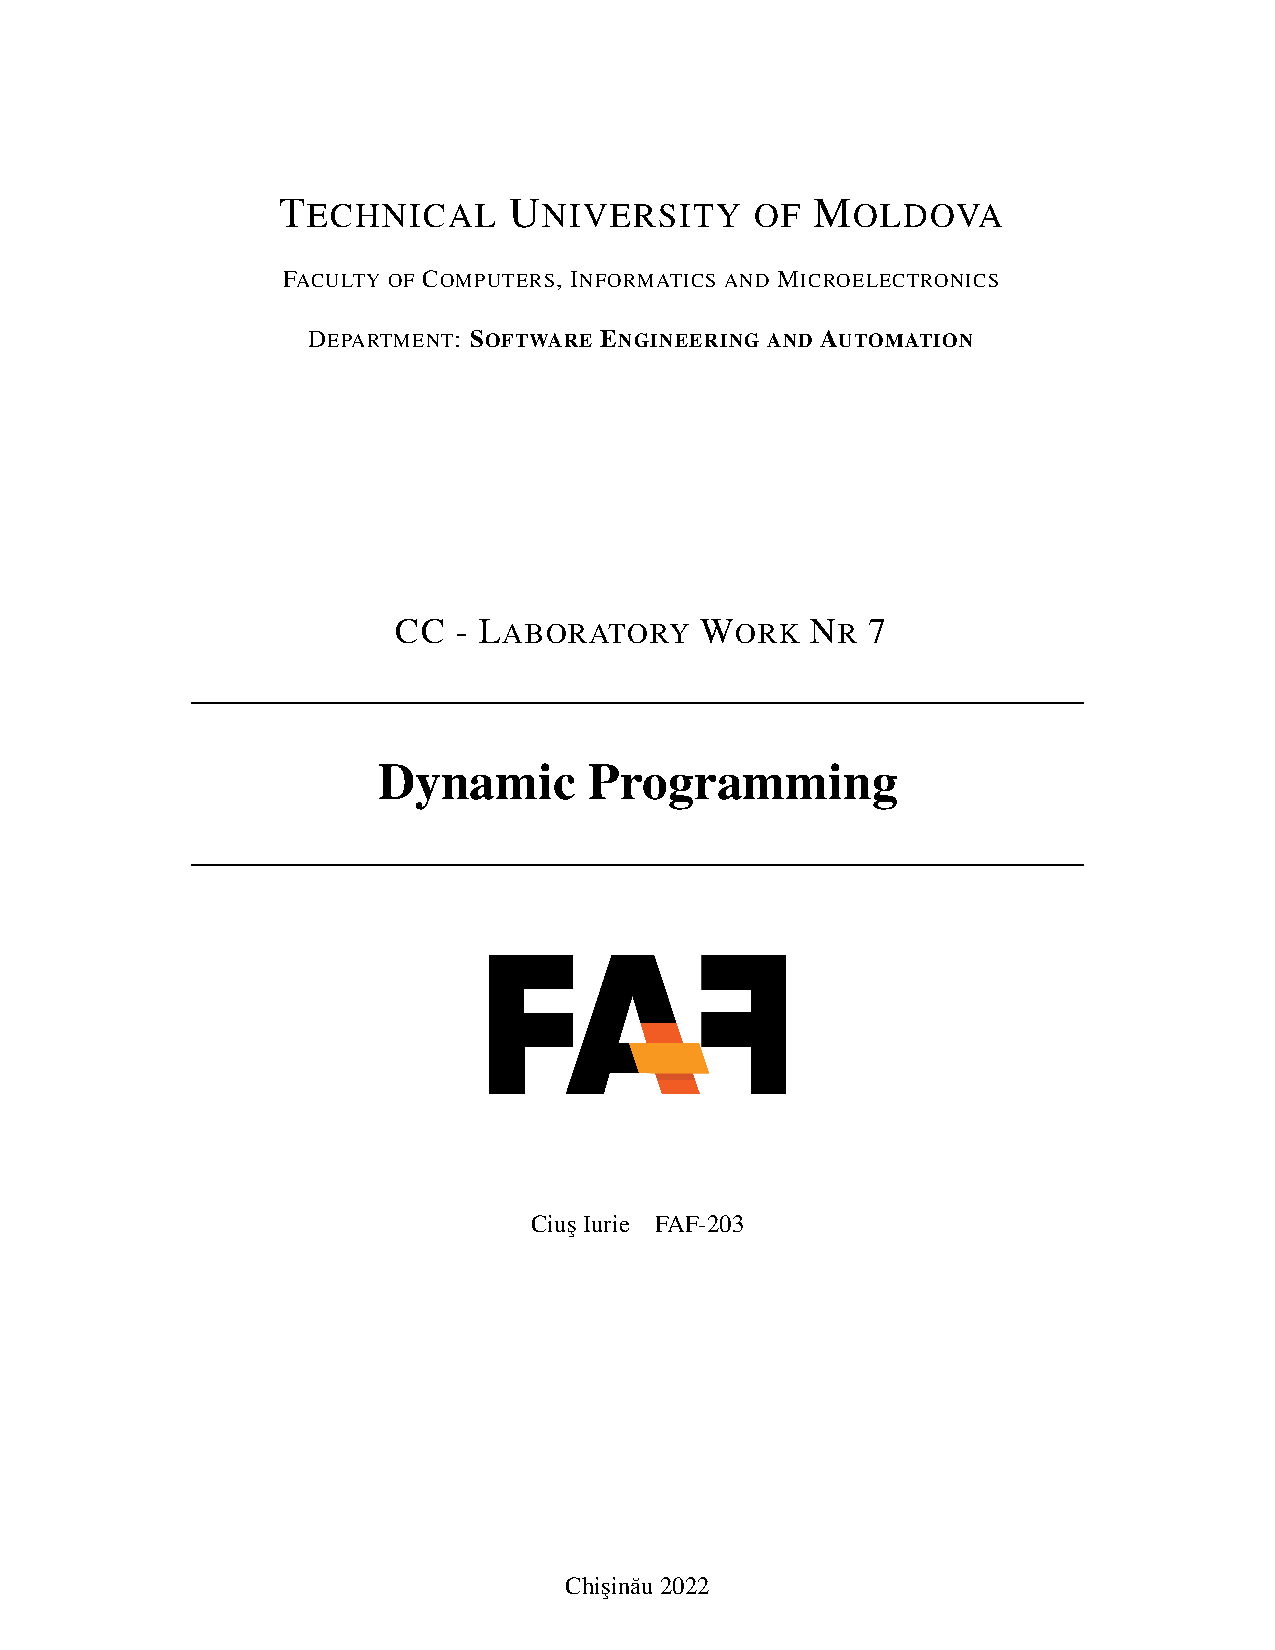
\includepdf[pages={1}]{title.pdf}
\tableofcontents

\newpage

\section{Algorithm Analysis}

\par Algorithm analysis is an important part of computational complexity theory, which provides theoretical estimation for the required resources of an algorithm to solve a specific computational problem. Analysis of algorithms is the determination of the amount of time and space resources required to execute it.

\subsection{Objectives}

\begin{itemize}
  \item Implement at least 3 algorithms that determine the N-th Fibonacci term.
  \item Establish the properties of the input data in relation to which the analysis is made.
  \item Choose the metric for comparing algorithms.
  \item Perform empirical analysis of the proposed algorithms.
  \item Make a conclusion on the work done.
\end{itemize}

\subsection{Introduction}

In mathematics, the \textbf{Fibonacci numbers}, commonly denoted $F_n$, 
form a sequence, the Fibonacci sequence, in which each number 
is the sum of the two preceding ones. The sequence commonly 
starts from 0 and 1, although some authors omit the initial 
terms and start the sequence from 1 and 1 or from 1 and 2. 
Starting from 0 and 1, the next few values in the sequence are:
$$0, 1, 1, 2, 3, 5, 8, 13, 21, 34, 55, 89, 144, ...$$

\par Fibonacci numbers appear unexpectedly often in mathematics, so much 
so that there is an entire journal dedicated to their study, the 
Fibonacci Quarterly. Applications of Fibonacci numbers include computer 
algorithms such as the Fibonacci search technique and the Fibonacci heap 
data structure, and graphs called Fibonacci cubes used for interconnecting 
parallel and distributed systems. They also appear in biological settings, 
such as branching in trees, the arrangement of leaves on a stem, the fruit 
sprouts of a pineapple, the flowering of an artichoke, an uncurling fern, 
and the arrangement of a pine cone's bracts. \par


Fibonacci numbers are strongly related to the golden ratio: 
Binet's formula expresses the \textit{nth} Fibonacci number in terms 
of n and the golden ratio, and implies that the ratio of two 
consecutive Fibonacci numbers tends to the golden ratio as n 
increases. Fibonacci numbers are also closely related to Lucas 
numbers, which obey the same recurrence relation and with the
Fibonacci numbers form a complementary pair of Lucas sequences.
\subsection{Theoretical Notes}

\subsubsection{Algorithm execution time}

Often, to solve a problem, one algorithm must be chosen from several possible ones,
two main selection criteria being contradictory:

\begin{enumerate}
  \item the algorithm should be easy to understand, code and troubleshoot.
  \item the algorithm to efficiently use computer resources, to have a short execution time.
\end{enumerate}

If the program being written has to be run a small number of times, the first requirement is more
importance; In this situation, the time to set up the program is more important than its time
so the simplest version of the program should be chosen.

If the program is to be run a large number of times, with a large number of data
processed, the algorithm that leads to a faster execution must be chosen. Even in this situation, it should
previously implemented the simplest algorithm and calculated the reduction of execution time that would
bring it the implementation of the complex algorithm.

The running time of a program depends on the following factors:

\begin{itemize}
  \item input data;
  \item the quality of the code generated by the compiler;
  \item the nature and speed of execution of the program instructions;
  \item the complexity of the algorithm that underlies the program.
\end{itemize}

So the running time is a function of its input, most of the time, not depending on the values from
input, but the number of data.

Next we will denote by \textit{T(n)} the execution time of an algorithm destined to solve a
size problems n. In order to estimate the execution time, a calculation model must be established and a
Unit. We will consider a computational model (also called a random access computing machine)
characterized by:

\begin{itemize}
  \item Processing is performed sequentially.
  \item Elementary operations are performed in constant time regardless of the value of the operands.
  \item The access time to the information does not depend on its position (there are no differences between the processing
  the first element and the last element of an array).
\end{itemize}

\textbf{The importance of the worst case scenario.} In the appreciation and comparison of algorithms, the most interesting
unfavorable case because it provides the longest execution time relative to any size input data
fixed. On the other hand, for some algorithms the worst case is relatively common

As for the analysis of the most favorable case, it provides a lower margin of time
execution and can be useful for identifying inefficient algorithms (if an algorithm has a high cost in the most
favorable case, then it cannot be considered an acceptable solution).

\textbf{Average execution time.} Sometimes extreme cases (the most unfavorable and the most favorable) are rare,
so the analysis of these cases does not provide enough information about the algorithm.

In these situations, another measure of the complexity of the algorithms is useful, namely the average execution time.
This represents an average value of the execution times calculated in relation to the probability distribution
corresponding to the input data space.

\newpage

\subsubsection{Empirical analysis of the complexity of algorithms}

An alternative to mathematical analysis of complexity is \textit{empirical analysis.}

This may be useful for: (i) obtaining preliminary information on the complexity class of a
algorithm; (ii) to compare the efficiency of two (or more) algorithms for solving the same
problems; (iii) to compare the efficiency of several implementations of the same algorithm; (iv) to
obtain information on the efficiency of implementing an algorithm on a particular computer.

\textbf{The stages of empirical analysis.} In the empirical analysis of an algorithm the following steps are usually followed:

\begin{enumerate}
  \item The purpose of the analysis is established
  \item Choose the efficiency metric to be used (number of executions of a / some operations or time
  execution of the whole algorithm or a part of the algorithm.
  \item The properties of the input data are established in relation to which the analysis is performed (data size
  or specific properties).
  \item The algorithm is implemented in a programming language.
  \item Multiple sets of input data are generated.
  \item The program runs for each input data set.
  \item The obtained data are analyzed.
\end{enumerate}

The choice of the efficiency measure depends on the purpose of the analysis. If, for example, the aim is to obtain
information on the complexity class or even checking the accuracy of a theoretical estimate then
it is appropriate to use the number of operations performed. If the goal is to assess behavior
implementation of an algorithm then is appropriate to the execution time.

To perform an empirical analysis is not enough a single set of input data but several, which
highlight different features of the algorithm. It is generally good to choose data
different sizes so as to cover the range of all dimensions that will appear in practice. On
on the other hand, the analysis of different values or configurations of the input data is also important. If so
analyzes an algorithm that verifies whether a number is prime or not and testing is done only for numbers
which are not prime or only for numbers that are prime then you will not get a relevant result.
The same thing can happen with a behavioral algorithm depending on the degree of sorting of one
array (if you choose only the array almost sorted according to the desired criterion or arrays ordered in reverse
analysis will not be relevant).

In order to empirically analyze the implementation of the algorithm in a programming language will need
introduced sequences whose purpose is to monitor execution. If the efficiency metric is the number of
executions of an operation then a counter is used which is incremented after each execution a
that operation. If the metric is the execution time then the time of entry must be recorded
the analyzed sequence and the time of exit. Most programming languages offer measurement functions
the time elapsed between two moments. This is especially important if you are active on your computer
several tasks, to count only the time allocated to the execution of the analyzed program. Especially if
it is about measuring the time it is indicated to run the test program several times and to
calculate the average value of time.

After the execution of the program for the test data the results are recorded and for the purpose of the analysis either
calculates synthetic quantities (mean, standard deviation, etc.) or plot pairs of points
shape (problem size, efficiency measure).

\newpage

\section{Code}

The following pages show my code implementation and result of the choosen algorithms.

\subsection{Implementation}

\subsubsection*{FIBONACCI.py}
\lstinputlisting[language=Python, linerange={1-26}]{../FIBONACCI.py}

\newpage

\lstinputlisting[language=Python, linerange={26-48}]{../FIBONACCI.py}

\newpage

\subsubsection*{App.py}
\lstinputlisting[language=Python]{../App.py}

\newpage

\subsection{Time Complexity}

\subsubsection*{Method 1 (Recursion)}

\textbf{\textit{Time Complexity:}} T(n) = T(n) which is linear. 

If the original recursion tree were to be implemented then this would have been the tree but now for n times the recursion function is called

Original tree for recursion

\begin{lstlisting}
                          fib(5)   
                     /                \
               fib(4)                fib(3)   
             /        \              /       \ 
         fib(3)      fib(2)         fib(2)   fib(1)
        /    \       /    \        /      \
  fib(2)   fib(1)  fib(1) fib(0) fib(1) fib(0)
  /     \
fib(1) fib(0)
\end{lstlisting}

Optimized tree for recursion for code above

\begin{itemize}
  \item fib(5) 
  \item fib(4)
  \item fib(3)
  \item fib(2)
  \item fib(1)
\end{itemize}

O(n) if we consider the function call stack size, otherwise O(1).

\subsubsection*{Method 2 (Dynamic Programming) }

For dynamic Programming, the time complexity would be O(n) since we only loop through it once. As you can see in the dynamic programming procedure chart, it is linear.

And the space complexity would be $O(N)$ since we need to store all intermediate values into our list. So the space we need is the same as n given.

\subsubsection*{Method 3 (Space Optimized Method 2) }

\textbf{Time Complexity:} O(n) \\
\textbf{Extra Space:} O(1)

\subsubsection*{Method 4 (Using formula) }

\textbf{Time Complexity:} O(logn) \\
\textbf{Extra Space:} O(1)

\subsection{Graphs}

\includegraphics[width=15cm]{graphs.png}

\newpage

\section{Conclusion}

The Fibonacci sequence may not be the perfect example 
for an in-depth understanding of dynamic programming. 
But it shows us the steps to convert a recursive solution 
into a dynamic programming solution. To start with the idea 
of dynamic programming, it is a simple and easy-to-understand 
example. We can expand our understanding of dynamic programming 
by solving problems like —
\begin{itemize}
  \item Longest Common Subsequence problem.
  \item Shortest Common Subsequence problem.
  \item 0/1 Knapsack problem.
  \item Matrix Chain Multiplication problem.
  \item Rod Cutting Problem.
\end{itemize}

We analyzed the time complexity of 4 different 
algorithms that find the nth value in the Fibonacci Sequence and plot 
the time versus the nth Fibonacci's number.

\subsection{References}

\begin{itemize}
  \item https://github.com/IuraCPersonal/CC
\end{itemize}

\end{document}

%=                END                      =%
%===========================================%